\section{Architecture}
In software engineering, the architecture refers to the high-level design that organizes a system's core elements. This includes, but is not limited to, components such as modules, packages, and programming languages. Key design decisions are involved which are essential for constructing a strong foundation to build off of, thus making it critical to have for successful future development. With this in mind, we have chosen to utilize a three-tier architecture. This will use JavaScript, React, and CSS for constructing the user interface, Java for the application, and Firebase as our database.

\begin{center}
    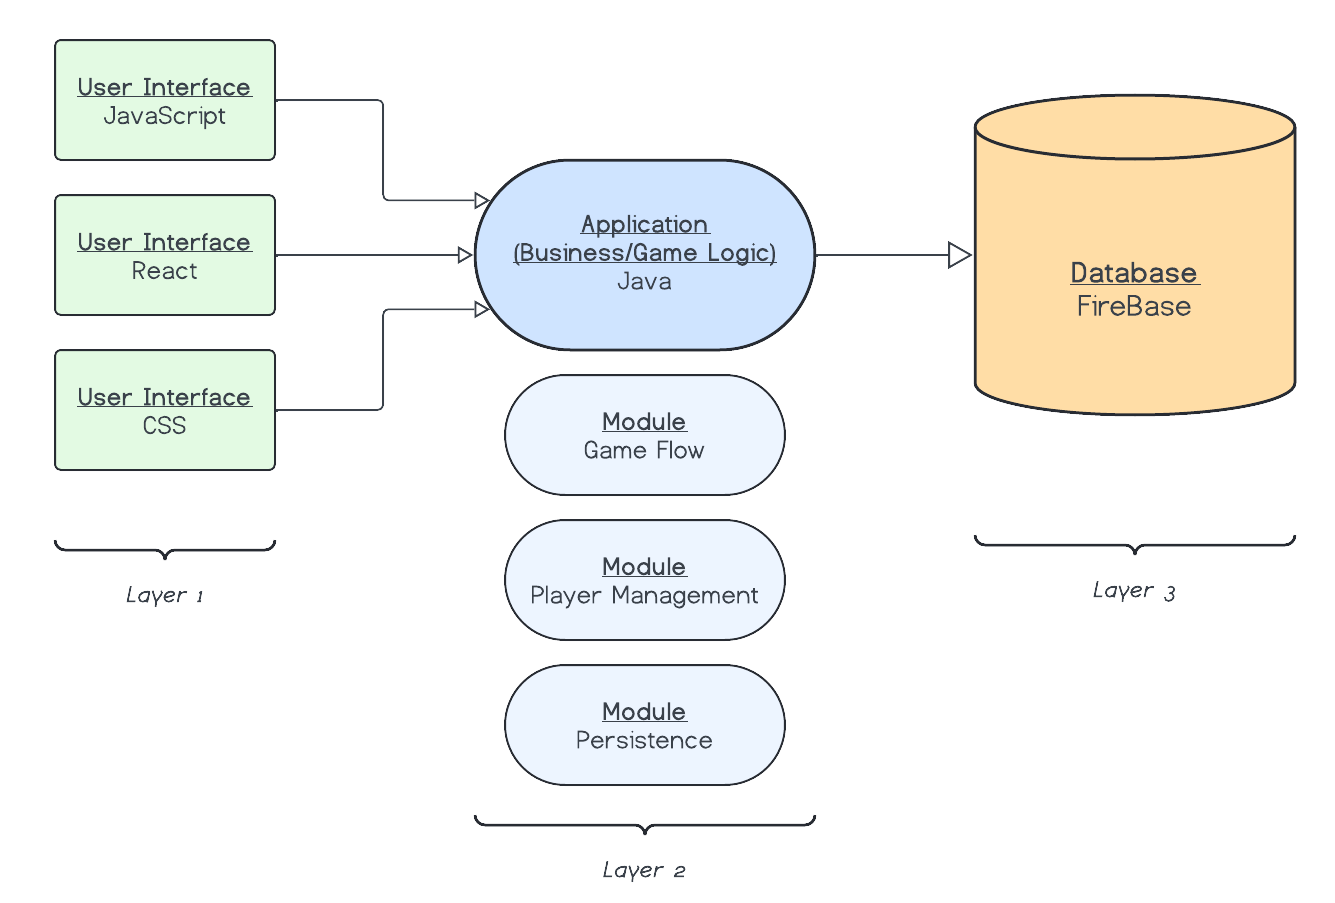
\includegraphics[scale=0.3]{CS482 Assignment 2 Architecture FINAL.png}
\end{center}

For our Go Fish application, we will utilize a three-tier architecture that is structured around user interface, application, and database. We have chosen this architecture because its components align with our goals in creating a card game web application that offers an enjoyable user experience in both visuals and playing the actual game. As seen in the figure above, it is made up of three distinct layers.

\subsection{User Interface}
Handling the display of game elements, user interaction, and input processing is essential for the frontend of a web application. We will be utilizing JavaScript, React, and CSS to do so. These languages will allow us to construct a well-designed UI to ensure a smooth and engaging experience for the user. The design emphasizes a classic card table feel with a responsive layout that adapts to various screen sizes. Cards are styled with consistent proportions, rounded corners, and a clear display for the suits and ranks of cards. The game board mimics a card table, featuring distinct player areas and a centralized deck. Interactive elements like hover effects on cards and smooth animations for card movements enhance user engagement.

\pagebreak

\subsubsection{Visual Design Draft}
\begin{enumerate}
    \item\textbf{Card Design}
    \begin{itemize}
        \item Card Size \& Proportions: Maintain a consistent aspect for the cards 
    
        \item Visual Components
        \begin{itemize}
            \item Suit \& Rank: Place the rank and suit symbol clearly in the top-left and bottom-right corners of each card
            \item Centered Design: Use the center of the card for the suit symbol
            \item Rounded Corners: Give the cards rounded corners for a modern look (use border-radius in CSS)
            \item Border: Add a subtle border around the cards to distinguish them from the background
        \end{itemize}
    \end{itemize}

    \item \textbf{Display for Hand of Cards}
    \begin{itemize}
        \item Grid Layout for Player's Hand: Use a horizontal layout for cards in a player’s hand
        \item Hover Effects: Make the cards interactive with hover effects
    \end{itemize}

    \item\textbf{Playing Table}
    \begin{itemize}
        \item Table Layout: The game area should mimic a table for cards
        \item Player Zones: Each player should have a distinct area where their hand of cards is displayed
        \item Center Game Elements: Ensure the draw pile or game deck is in the center of the table
    \end{itemize}

    \item\textbf{Visual Aesthetics}
    \begin{itemize}
        \item Color Scheme: Use a color palette that is easy on the eyes and give it a classic card table feel
    \end{itemize}

    \item\textbf{Animations \& Transitions}
    \begin{itemize}
        \item Card Movement: When a card is drawn or played, add subtle animations to make the movement more engaging
        \item Transition for Cards: Use smooth transitions for flipping cards or drawing them from the deck
    \end{itemize}

    \item\textbf{Responsive Design}
    \begin{itemize}
        \item Ensure the game layout is responsive for various screen sizes like desktops to mobile devicesk
    \end{itemize}
    \pagebreak

    \item\textbf{Player Information Display}
    \begin{itemize}
        \item Player Avatars and Names: Display player avatars or profile pictures next to their card area for personalization
    \end{itemize}
\end{enumerate}

Overall, the design prioritizes user experience, blending classic card game elements with modern web design principles to create an  enjoyable game of Go Fish for the players.

\subsection{Application}
The application layer will involve several key modules that are crucial for the actual game rules. The player management module will handle everything related to the player, such as storing and managing player profile information or managing each player’s hands during games. The game flow module is responsible for the actual gameplay mechanics of Go Fish in terms of ensuring each player’s turn runs accordingly based on the real card game. Finally, we have the persistence module which ensures that database operations (such as saving or retrieving game states) are abstracted from other parts of the business logic. 

\subsection{Database}
In the third layer, we will be implementing Firebase as our database for storing all sorts of data that is to be manipulated by the system. For example, once a game of Go Fish is completed, each player’s information is updated in the database in terms of their wins/losses and amount of virtual currency.